% Chapitre 02 : Etat de l'art
\chapter{Une approche tridimensionnelle pour le diagnostic du cancer de la prostate}\label{chapter:02:presentation_probleme}
{
	
	% Intro chap2 {{{
	De nos jours, les diagnostics du cancer de la prostate sont effectués en utilisant une échelle histologique 2D appelée échelle de Gleason~\cite{cite_gleason_score}. Cette échelle permet de reconnaître le stade d'avancement de la maladie selon les formes des glandes dans un échantillon de prostate en  comparant une image d'une coupe 2D à une approximation graphique faite par Dr. \textsc{Gleason} (voir \ref{section:gleason_scale}). L'utilisation de cette échelle %ne permet pas un diagnostic précis 
	entraîne une variabilité de diagnostic importante car dépendante de l'orientation de la coupe 2D. C'est pour cela que des méthodes de diagnostics utilisant de l'information tridimensionnelle sont en cours de développement.
	%L'équipe de bio-ingénierie de l'université de Tulane a développé une méthode d'imagerie permettant de reconstruire un échantillon en trois dimensions. Appliqué au diagnostic du cancer de la prostate, nous pourrons analyser la morphologie tridimensionnelle des glandes, encore inconnue. L'objectif est de mettre en place une méthode de diagnostic pouvant accompagner les méthodes actuelles telles que l'échelle de Gleason, pour enrichir les méthodes de diagnostic du cancer de la prostate. Notre tâche est de reconstruire cet échantillon rapidement et de manière fiable, à partir des images extraites de leur processus d'acquisition.
	% }}}
	
	Cette section présente la technique d'imagerie 3D développée à l'université de Tulane ainsi que le jeu de donnée résultant que nous avons à disposition.
	
	% Section Gleason {{{
	\section{L'\'echelle de Gleason}\label{section:gleason_scale}
	{
        % IMG : Echelle de Gleason {{{
		\begin{figure}[!h]
		    \centering
		    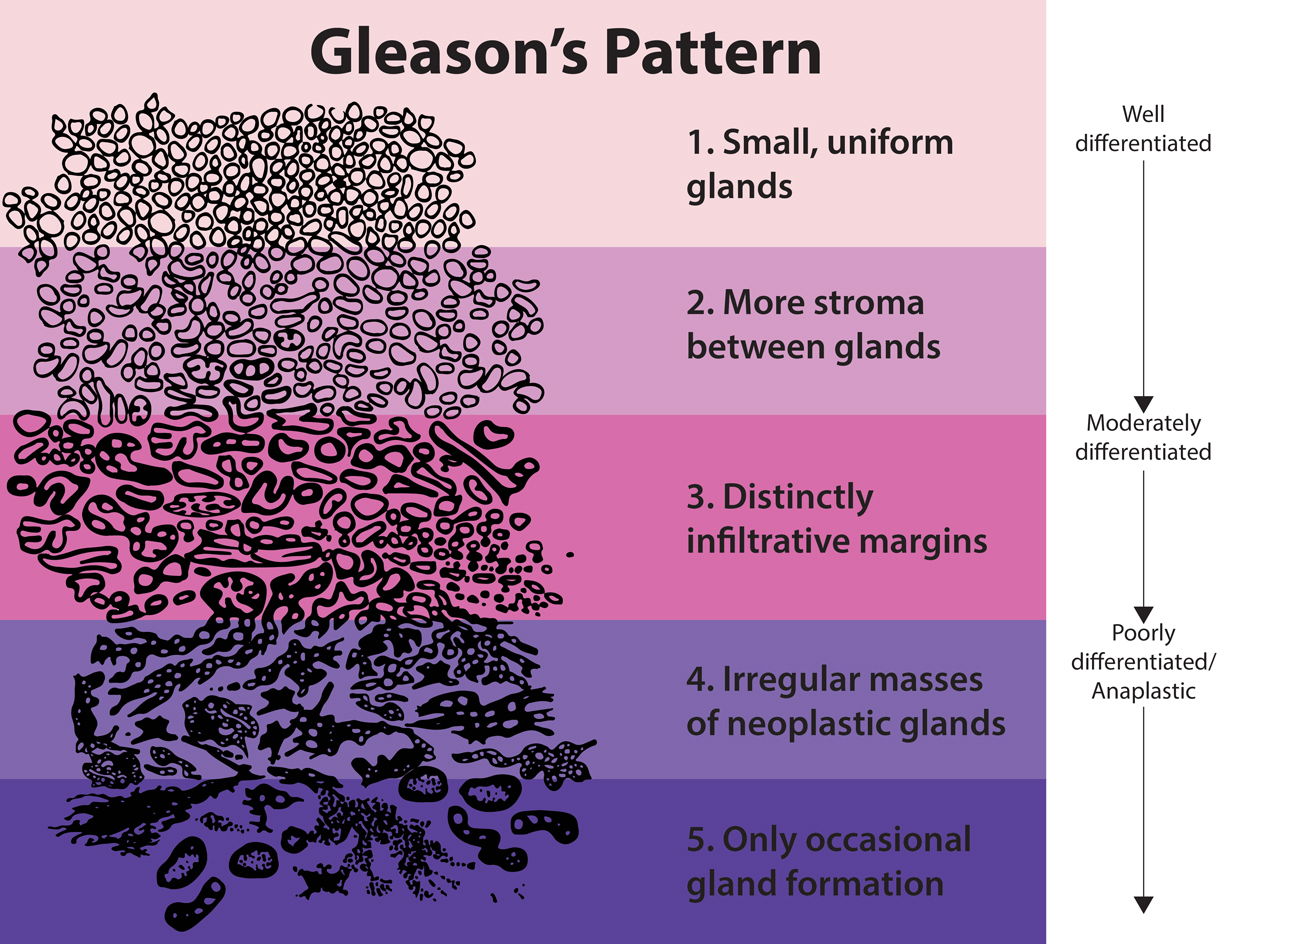
\includegraphics[width=.7\linewidth]{img/gleason_score.jpg}
		    \captionsetup{width=.8\linewidth}
		    \caption{L'échelle de Gleason, représentée schématiquement}
		    \label{img:gleason_scale}
		\end{figure}
		% }}}

		L'échelle de Gleason~\cite{cite_gleason_score} est une échelle pronostique qui se base sur l'observation de la forme des glandes d'une prostate afin d'évaluer la possibilité de présence d'un cancer chez un patient. Inventée par Donald \textsc{Gleason} entre 1960 et 1970, elle permet une évaluation de la présence et de l'avancement du développement d'un cancer de la prostate chez un individu. Cette échelle permet d'attribuer un score de 1 à 5 en fonction de la forme des glandes dans une coupe histologique de la prostate (voir figure \ref{img:gleason_scale}) par rapport à un diagramme fait par Dr.\textsc{Gleason} lors de ses recherches.

		Étant donné que cette échelle se base sur l'observation de coupes histologiques de la prostate, la direction des coupes, l'angle de celles-ci, ainsi que leur orientation influent beaucoup sur la forme observée des glandes de la prostate et donc sur le pronostic final donné par un médecin après observation (voir figure \ref{img:gleason_bias}).

		Afin de pallier cette incertitude, une des méthodes proposée par nos collaborateurs à la Nouvelle-Orléans consiste à analyser la morphologie tridimensionnelle des glandes. En effet, grâce à la méthode de microscopie \textit{di-SPIM}, nous pouvons obtenir une pile de coupes d'un échantillon permettant de construire une grille volumique le représentant. L'élaboration d'une méthode utilisant la morphologie tridimensionnelle des glandes pourrait permettre d'enrichir les connaissances liées à la détection du cancer de la prostate afin de détecter la pathologie plus rapidement, permettant de mieux la traiter par la suite. Une telle méthode viendrait étoffer les méthodes de diagnostic actuelles de détection du cancer de la prostate.
	}
	% }}}

	% Section microscopie {{{
	\section{Microscopie LSFM \& SPIM}\label{section:microscopy}
	{
		La microscopie \textit{LSFM}~\cite{cite_lsfm_explication_girard}, pour \textit{Light-Sheet Fluorescence Microscopy} ou microscopie par fluorescence à feuille de lumière en français est une méthode d'acquisition d'images. Elle consiste à illuminer une tranche de l'échantillon à analyser une fois rendu transparent perpendiculairement à l'axe du système de détection du microscope. La fluorescence de l'échantillon est alors un indicateur du tissu analysé. Plusieurs variations de la méthode existent, notamment une alternative appelée \textit{SPIM}~\cite{cite_spim_explication_original} : \textit{Single Plane Illumination Microscopy}, ou microscopie par éclairage planaire sélectif en français. Cette méthode permet de faire des acquisitions d'échantillons par pile de coupes rapidement, et permettant par la suite une reconstruction 3D de ceux-ci.

        % IMG : SPIM processus capture {{{
		\begin{figure}[!h]
			\centering
			
\includegraphics[width=0.5\linewidth]{./img/lsm_methode_01.jpg}
			\captionsetup{width=.8\linewidth}
			\caption{Processus d'acquisition par \textit{SPIM} : un rayon lumineux (en bleu) est envoyé dans l'échantillon, et la fluorescence de celui-ci est détectée par le dispositif de détection dans sa zone focale (en jaune)}
			\label{img:lsm_01_how_it_works}
		\end{figure}
		% }}}

		Tout comme la méthode \textit{LSFM}, la méthode \textit{SPIM} utilise la fluorescence d'un échantillon afin de l'analyser. Toutefois, la méthode SPIM utilise un éclairage latéral, ce qui permet de rendre les dispositifs d'éclairage et d'acquisition complètement indépendants.

		Les acquisitions sont faites grâce à des émissions de lumière dans l'échantillon à analyser. Ceci entraîne un problème : l'image d'un point de l'échantillon dans l'acquisition s'étale le long de l'axe d'émission. Cela cause une anisotropie\definition{L'anisotropie entraîne des propriétés différentes selon des directions différentes} de la fonction d'étalement de point\footnote{Réponse impulsionnelle d'un système d'imagerie à une source ponctuelle.} du capteur sur son axe dans l'acquisition par coupe d'un échantillon avec la méthode \textit{SPIM} (figure \ref{img:spim_01_point_spread_function}). Pour pallier ce problème, il existe une alternative à la méthode \textit{SPIM}, appelée \textit{di-SPIM}, pour \textit{dual inverted SPIM}. Cette variation consiste à utiliser en tandem deux dispositifs \textit{SPIM} afin d'éliminer l'anisotropie qui existe avec les méthodes de \textit{SPIM} traditionnelles. Un dispositif \textit{di-SPIM} est illustré en figure \ref{img:lsm_02_device}.

        % IMG : Photo microscope {{{
		\begin{figure}[!h]
			\centering
			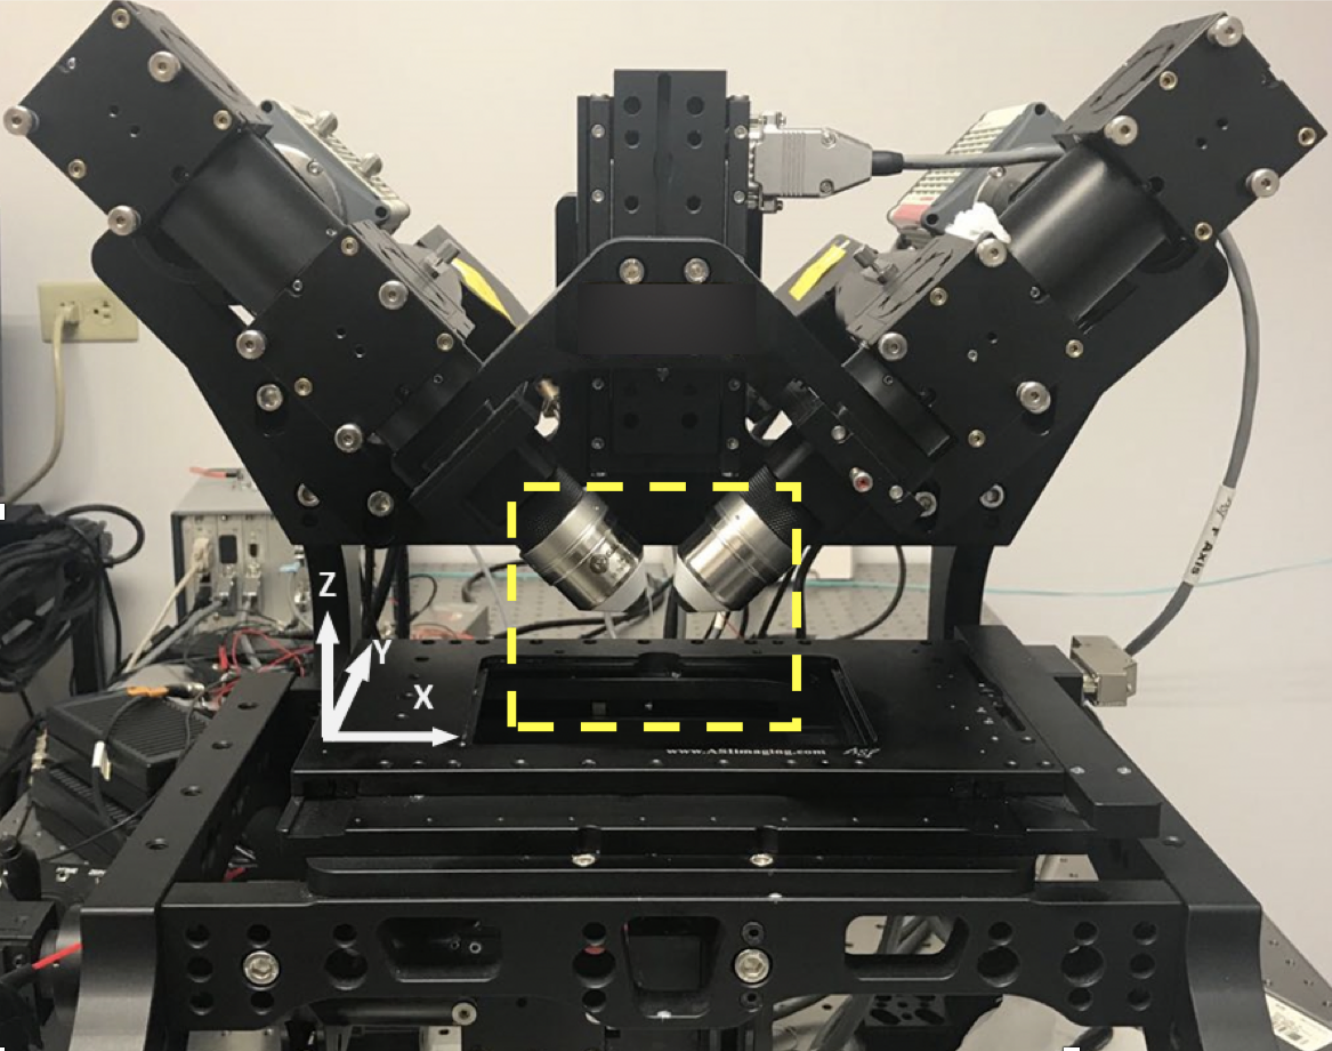
\includegraphics[width=0.5\linewidth]{./img/lsm_device_02.png}
			\captionsetup{width=.8\linewidth}
			\caption{Le microscope \textit{diSPIM} conçu par les chercheurs de la Nouvelle-Orléans permettant une acquisition tridimensionnelle d'un échantillon de manière fiable et rapide.}
			\label{img:lsm_02_device}
		\end{figure}
		% }}}

        % IMG : Fonction point étalement {{{
		\begin{figure}[!h]
			\centering
			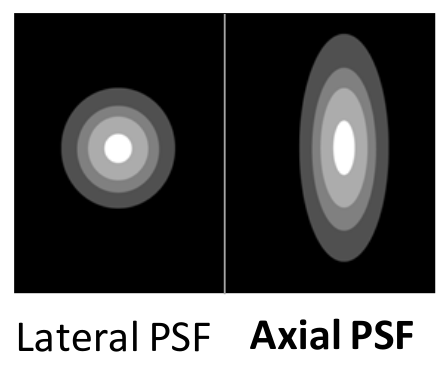
\includegraphics[width=0.3\linewidth]{./img/spim_01_psf.png}
			\captionsetup{width=.8\linewidth}
			\caption{Une image des fonctions d'étalement de point (PSF) axiales et latérales en imagerie SPIM.}
			\label{img:spim_01_point_spread_function}
		\end{figure}
		% }}}

		% IMG : Configurations SPIM, schéma {{{
		\begin{figure}[!h]
		    \centering
		    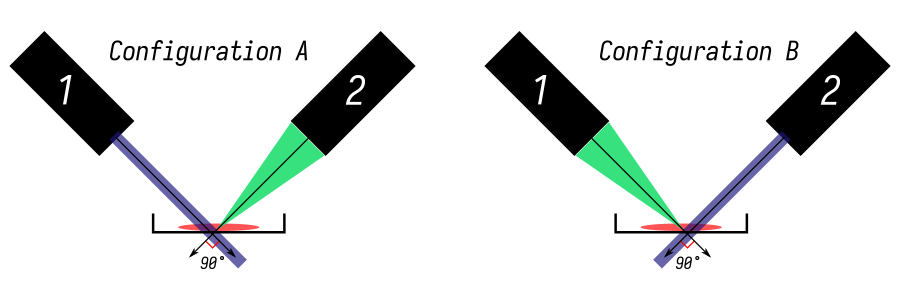
\includegraphics[width=.9\linewidth]{img/config_spim.png}
		    \captionsetup{width=.8\linewidth}
		    \caption{Configurations possibles des capteurs \textit{SPIM} (simplifié). En orange, l'échantillon reposant dans un récipient quelconque. En configuration A, la capteur 1 sert d'émetteur de lumière, et le capteur 2 sert d'appareil de capture. En configuration B, les rôles sont inversés.}
		    \label{img:spim_config}
		\end{figure}
		% }}}

		Dans cette méthode, il existe donc deux dispositifs \textit{SPIM} qui servent tour à tour de capteur, puis d'émetteur. Ces deux dispositifs sont placés à angle droit l'un de l'autre (voir figures \ref{img:lsm_02_device} et \ref{img:spim_config}), au dessus de la plateforme sur laquelle on dépose l'échantillon transparisé à analyser. Le fait d'avoir deux dispositifs \textit{SPIM} permet d'éliminer l'anisotropie de la fonction d'étalement de point dans les captures en combinant les acquisitions des capteurs depuis leurs points de vue différents, grâce à l'utilisation d'une opération de déconvolution\definition{Opération visant à restaurer le signal originel à une acquisition}.
		
		Le microscope \textit{di-SPIM} enregistre donc chacune des acquisitions d'un capteur dans une pile de coupes, qui sont discrétisées, quantifiées et enregistrées en tant qu'images traditionnelles au format \texttt{TIFF}, et qui nous est ensuite remise pour l'analyser et reconstruire un modèle tridimensionnel par la suite.
	}
	% }}}
	
	
    % Section jeux de données {{{
    \section{Présentation du jeu de données}\label{section:dataset}
    {
        Comme expliqué dans la section précédente, le microscope de l'université de Tulane possède deux capteurs disposés en angle droit l'un par rapport à l'autre. Ainsi, lors d'une acquisition d'un échantillon, le microscope capture des coupes à $\pm~\ang{45}$ par rapport à l'échantillon. Pour le système d'acquisition du microscope, cet échantillon est un signal continu tridimensionnel, comme représenté dans la figure \ref{img:spaces_real_initial}\texttt{(A)}. Ainsi, afin d'être enregistré, puis par la suite analysé il faut tout d'abord faire une discrétisation de ce signal, suivie d'une quantification de celui-ci. Ces deux étapes sont dépendantes des caractéristiques techniques du capteur (figure \ref{img:spaces_real_initial}\texttt{(B)}). Les images sont ensuite enregistrées sur disque, ce qui équivaut à leur appliquer une transformation (cisaillement) qui les place dans un repère orthonormé (voir figure \ref{img:spaces_real_initial} \texttt{(C)}). Dans cette configuration, l'échantillon est effectivement déformé par la transformation subie lors de l'enregistrement des images. Afin de le reconstruire, il nous sera nécessaire d'inverser cette transformation.

        Ces paires d'empilements d'images forment les différents jeux de données qui seront mis à notre disposition. Le microscope étant toujours en développement, ses caractéristiques techniques peuvent encore changer. La résolution des capteurs ainsi que le degré d'agrandissement fourni par le système optique pouvant évoluer dans le futur, il nous faudra pouvoir nous adapter à un tel changement.

        \begin{figure}[h]
            \centering
            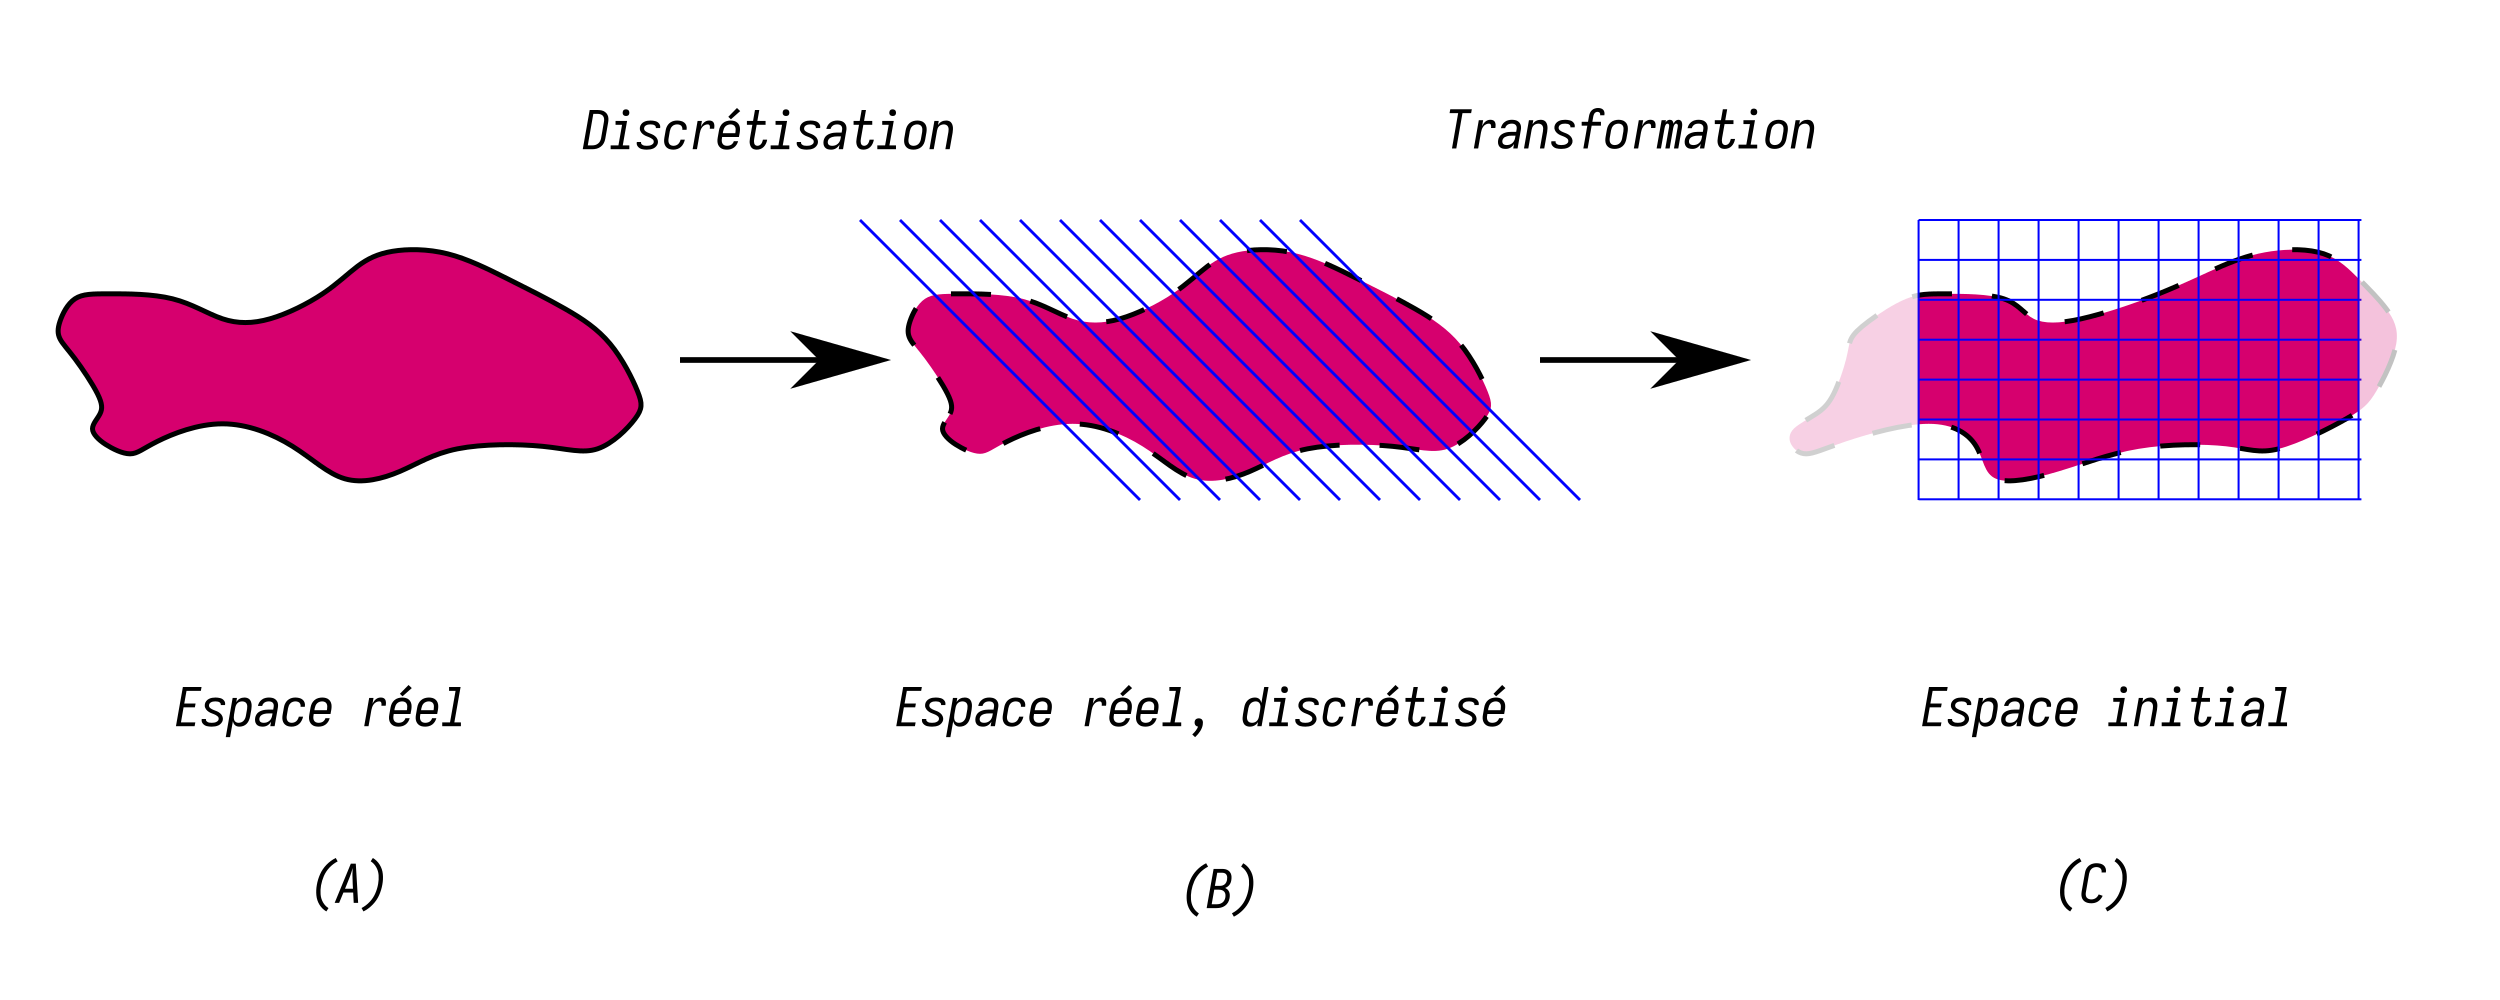
\includegraphics[width=\linewidth]{img/spaces_transfo_1_updated.png}
            \captionsetup{width=.8\linewidth}
            \caption{Différents espaces et transformations définis pour le programme. En magenta, l'échantillon à analyser. En bleu au centre, les différentes prises de vues effectuées par un capteur sur cet échantillon. En bleu à droite, la pile d'images résultante.}
            \label{img:spaces_real_initial}
        \end{figure}

        Afin de capturer un échantillon, le microscope effectue un ou plusieurs "balayages" du tissu (un exemple de plusieurs balayages est conceptualisé en figure \ref{img:multiple_image_captures}), afin de acquérir la totalité de celui ci. Chacune de ces captures sont constitués de deux piles d'images. En effet, comme vu en section~\ref{section:microscopy} la méthode de \textit{di-SPIM} utilise deux capteurs, orientés perpendiculairement l'un par rapport à l'autre. Le microscope est capable de prendre des acquisitions de l'échantillon contenant jusqu'à 20000 prises de vues. Ainsi, nous devons proposer des méthodes de traitement des données pour la visualisation et la reconstruction adaptées à ces jeux de données massifs.

        \begin{figure}[h]
            \centering
            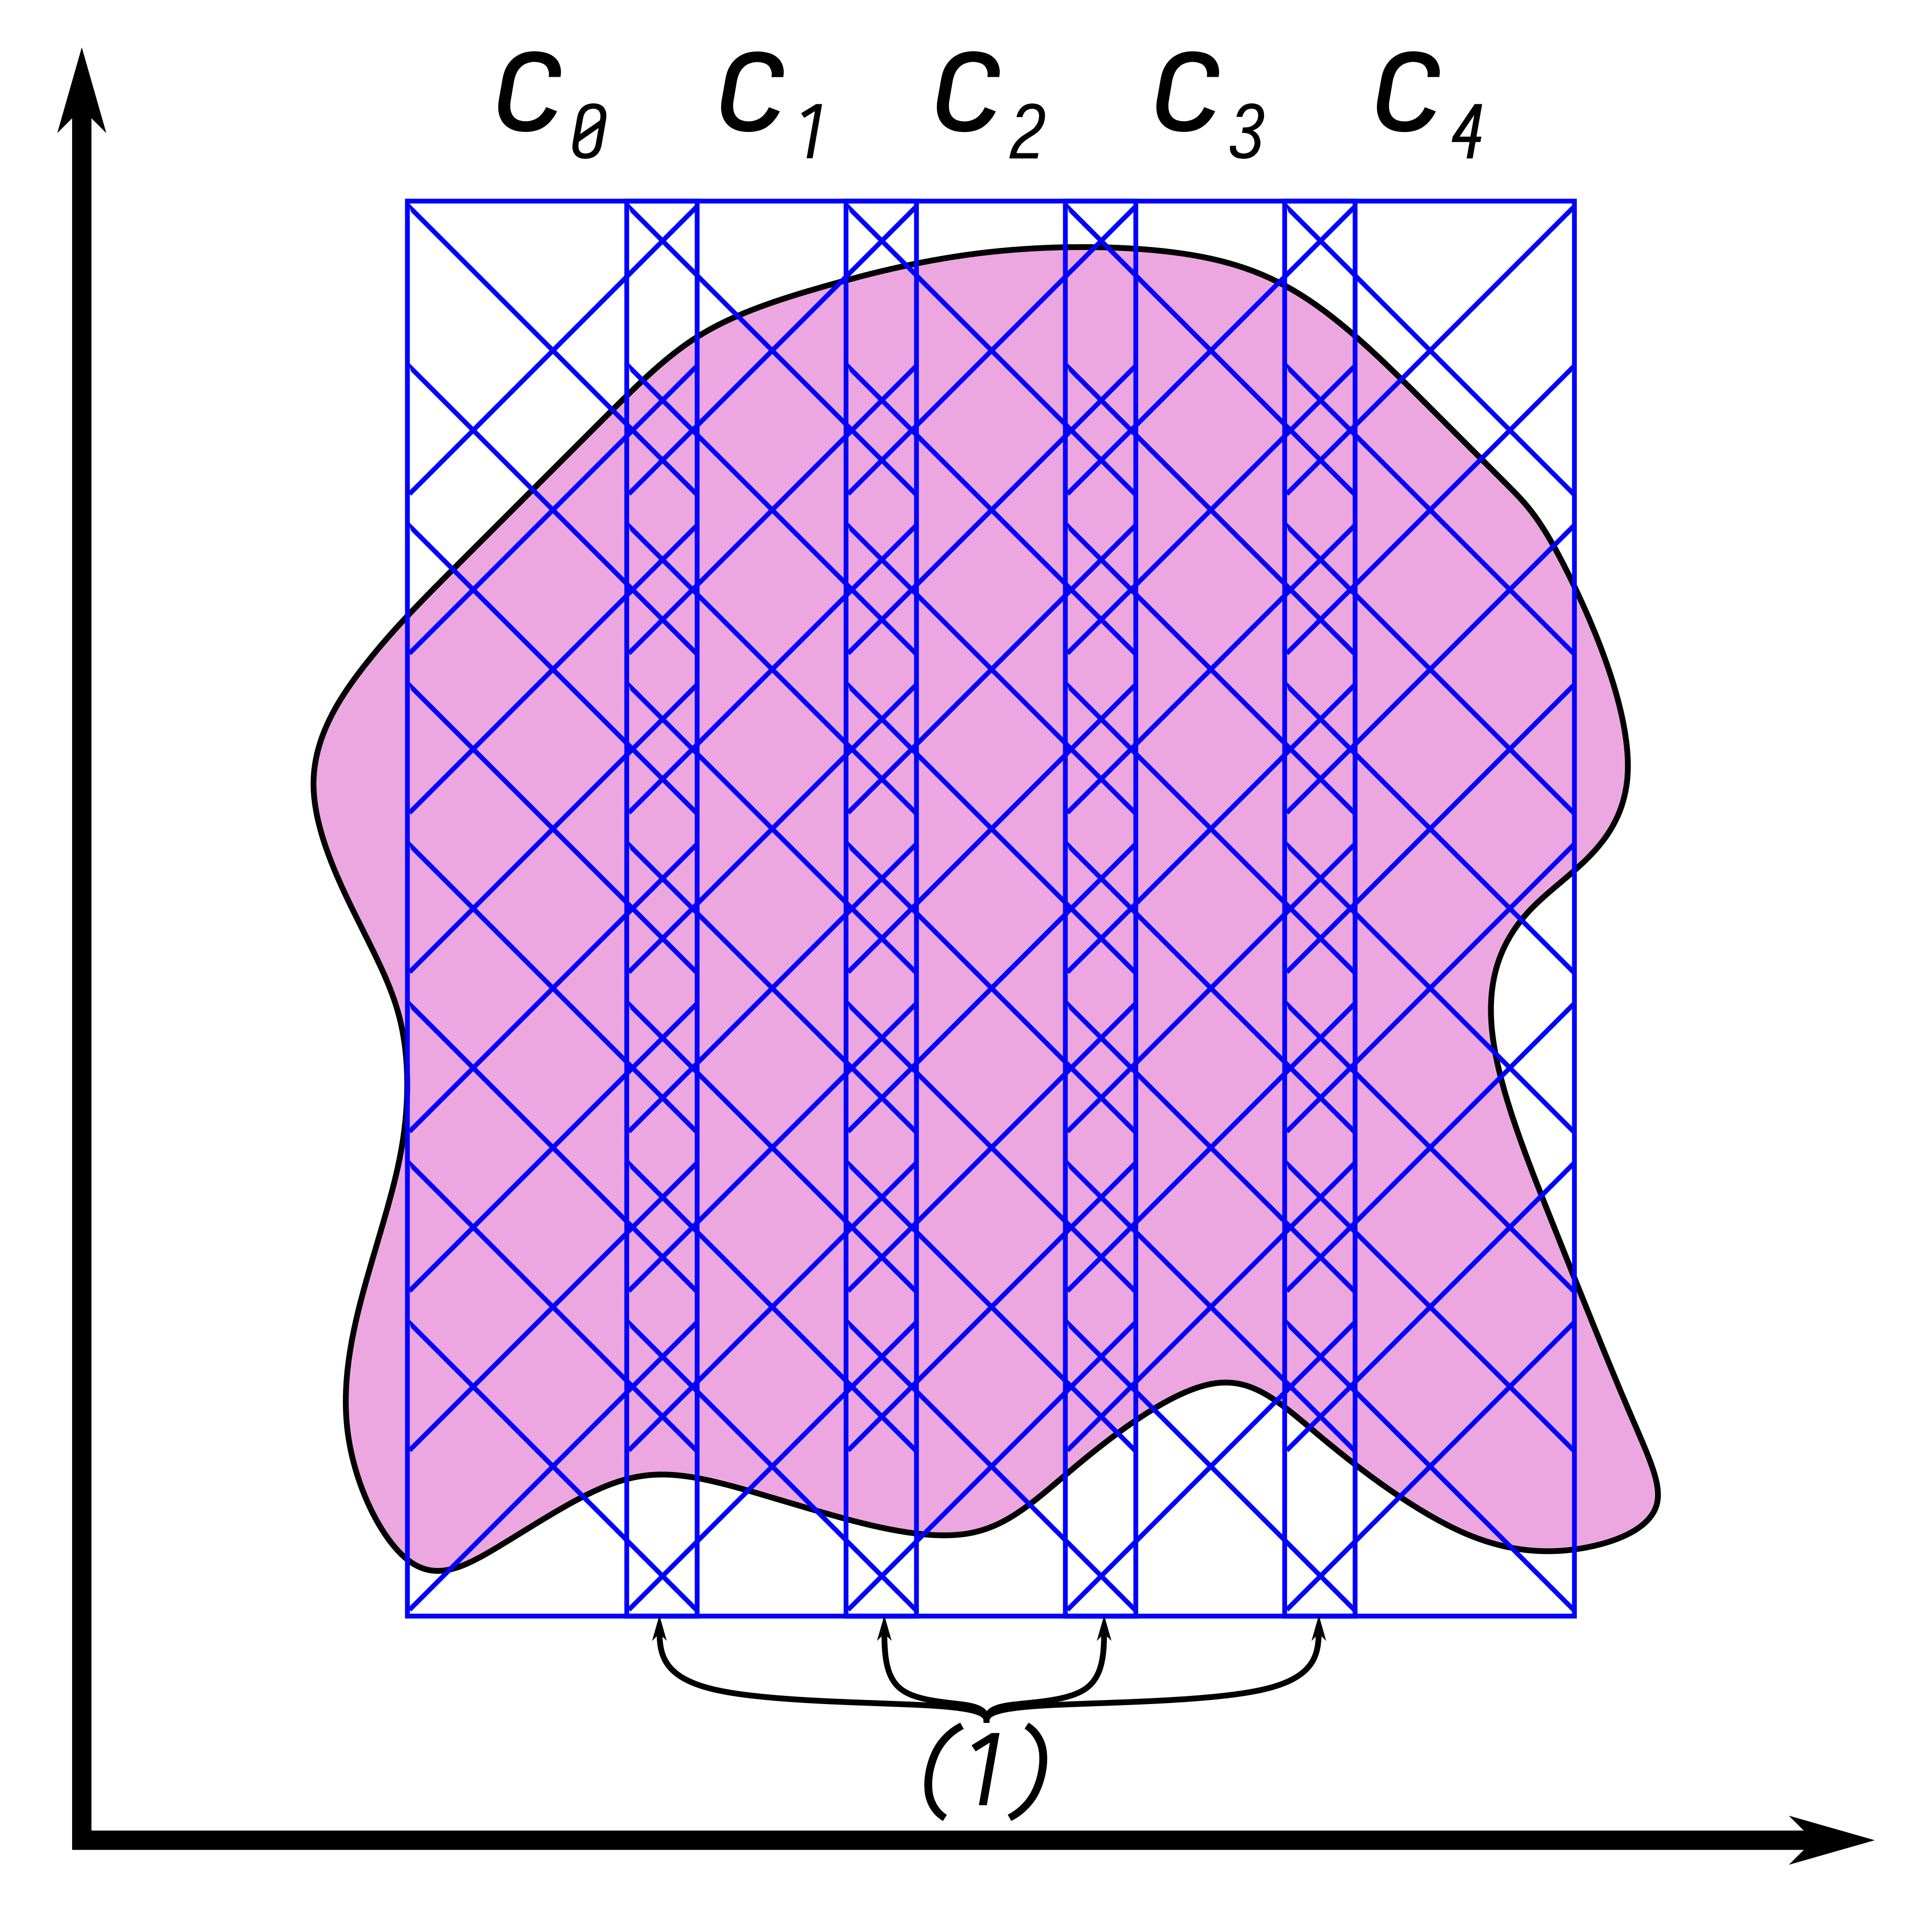
\includegraphics[width=.5\linewidth]{img/multiple_captures.png}
            \captionsetup{width=.7\linewidth}
            \caption{Un exemple d'acquisition d'un échantillon via de multiples captures. Chacune de ces captures (de $c_0$ à $c_4$) produira deux piles de $n$ images. Les captures présenteront des zones de chevauchement comme montré en (1).}
            \label{img:multiple_image_captures}
        \end{figure}

        Nous travaillons sur un jeu de données résultant d'une acquisition de tissu de prostate, composé d'une paire de piles d'images de 2000 images chacune. Les images sont de résolution $2048~\times~2048$, et sont en niveaux de gris sur 8 bits, résultant en une acquisition d'environ 16 gigaoctets. Ces piles d'images sont séparées en plusieurs fichiers \texttt{TIFF} contenant chacun une coupe uniquement. Un exemple d'un de ces fichiers peut être visualisé en figure \ref{img:data:both_prostate_samples}.

        \begin{figure}[ht]
            \centering
            \begin{tabular}{ccc}
                \begin{subfigure}[t]{.45\linewidth}
                    \centering
                    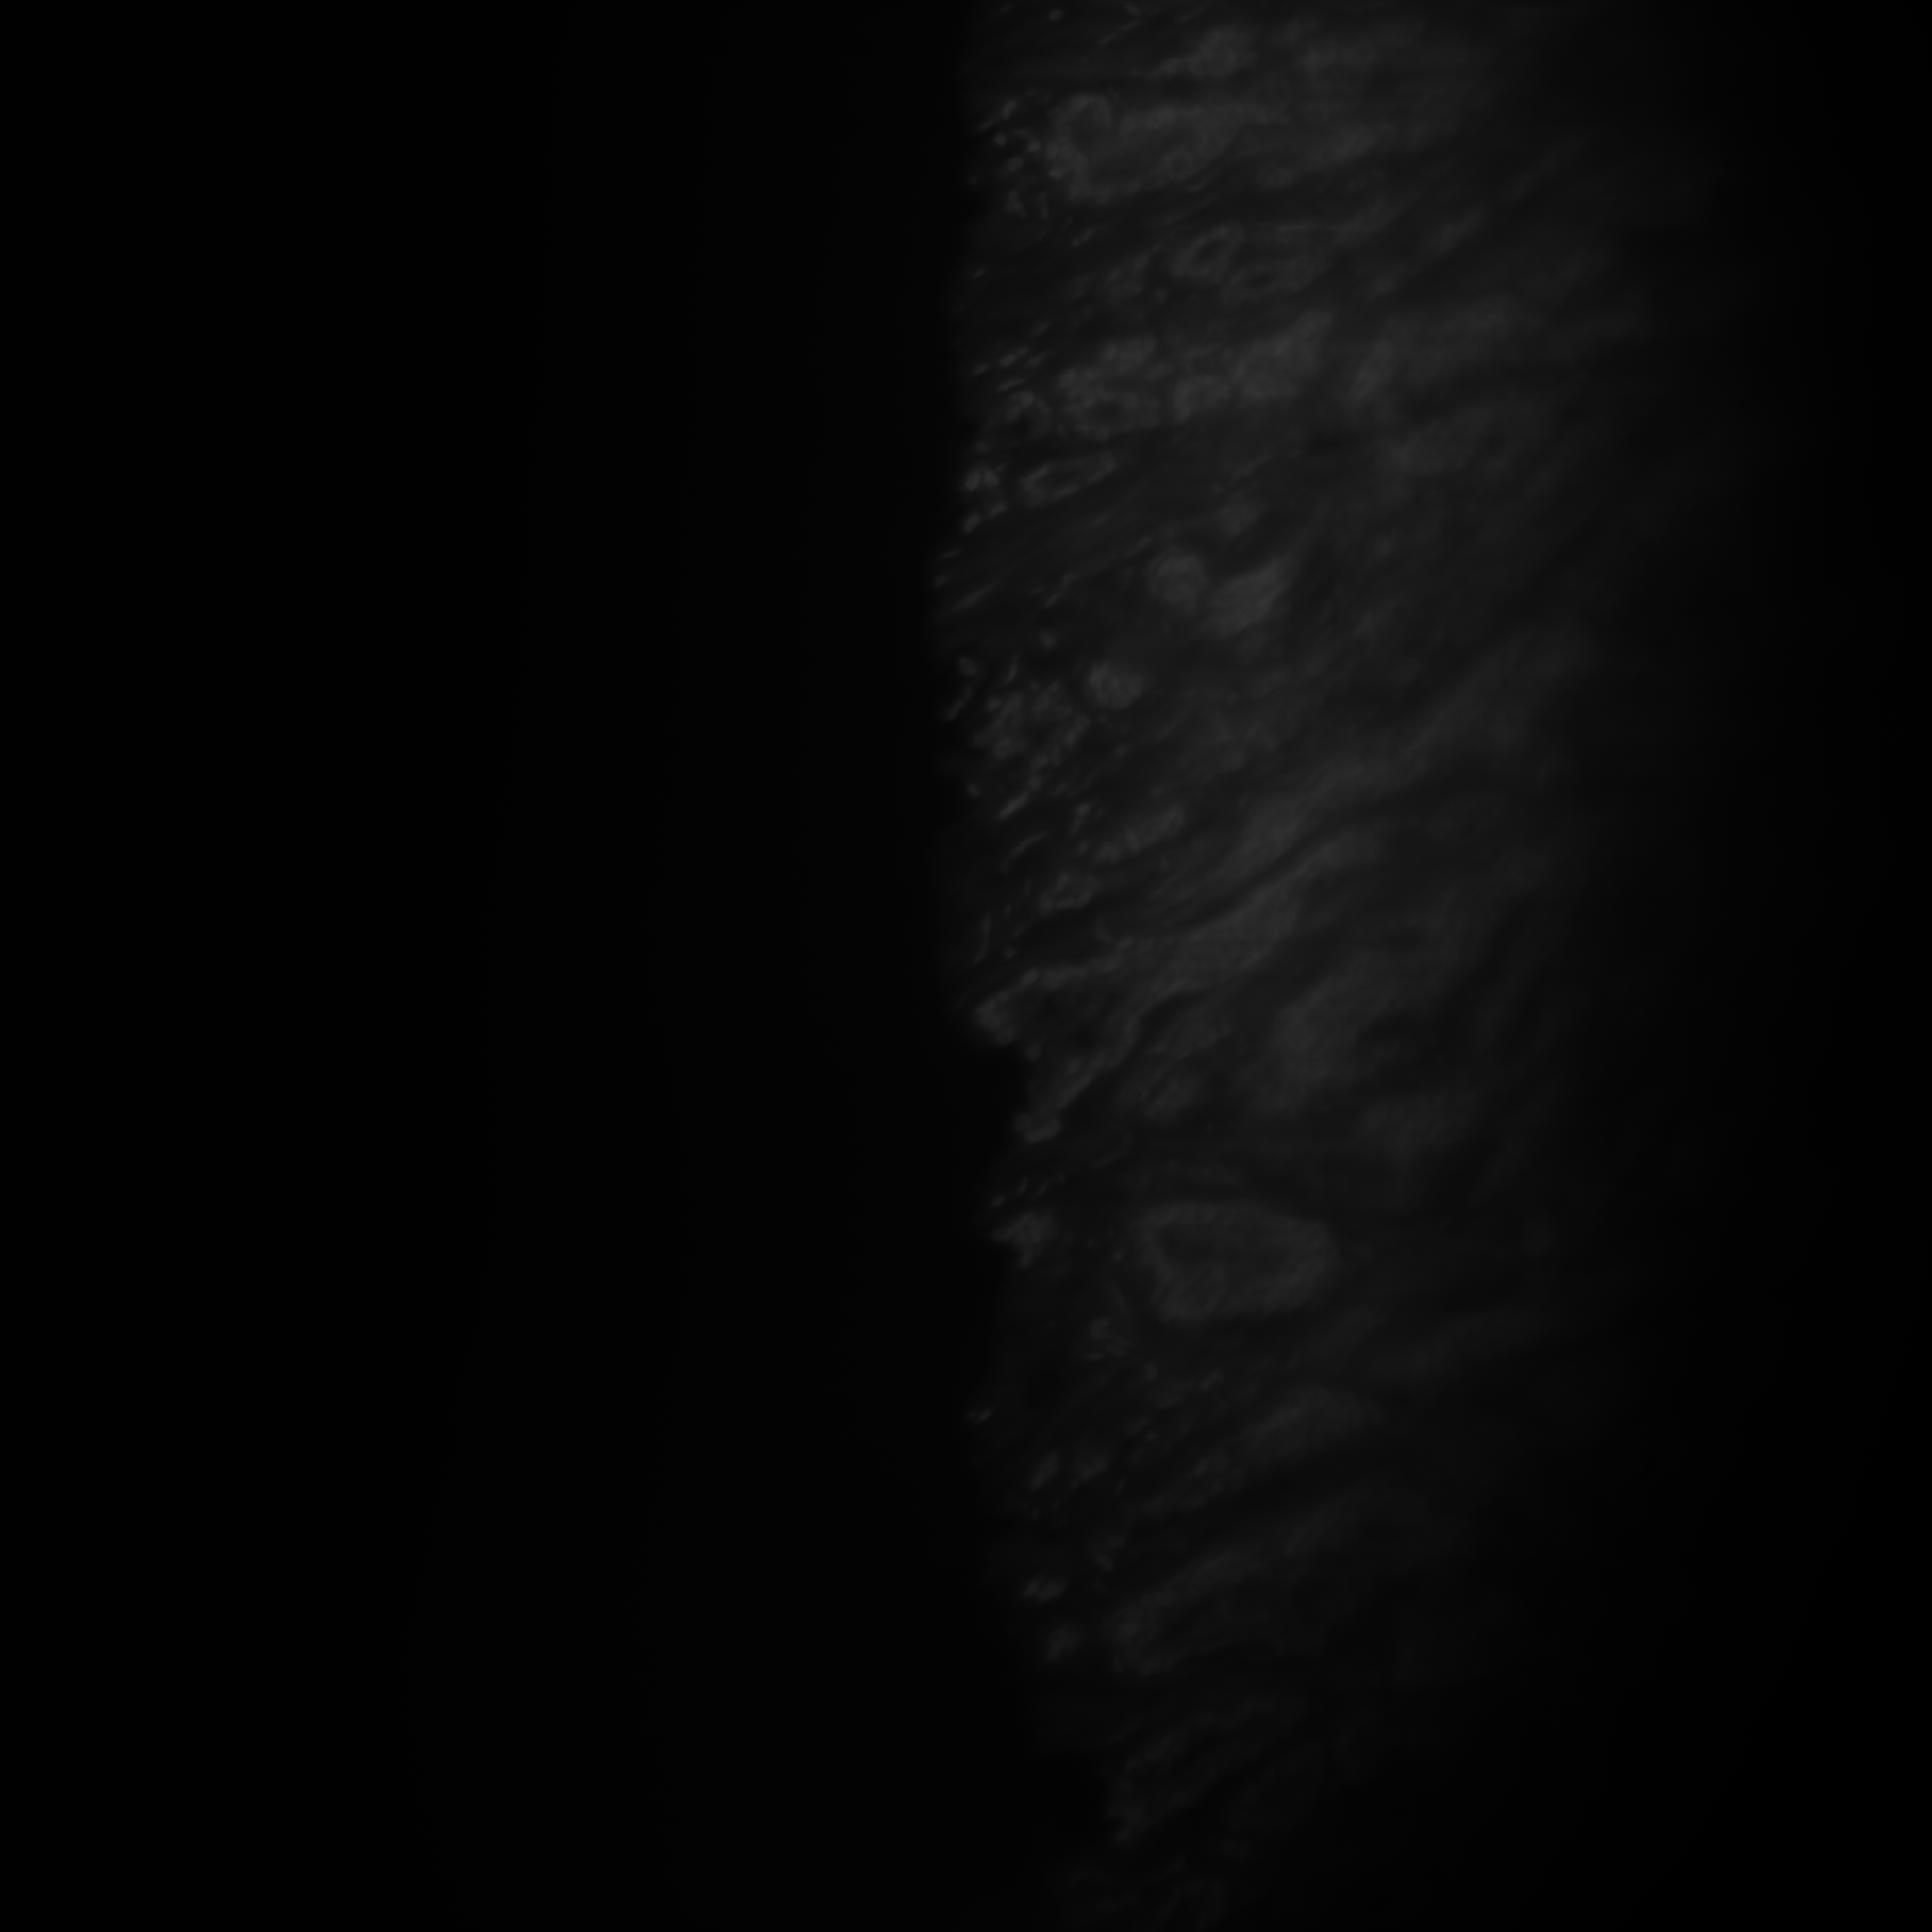
\includegraphics[width=.8\linewidth]{img/tulane_data/prostate_tulane.png}
                    \captionsetup{width=.8\linewidth}
                    \caption{Tissus de prostate, tels que capturés depuis le microscope}
                    \label{img:data:prostate}
                \end{subfigure}& \hfill &
                \begin{subfigure}[t]{.45\linewidth}
                    \centering
                    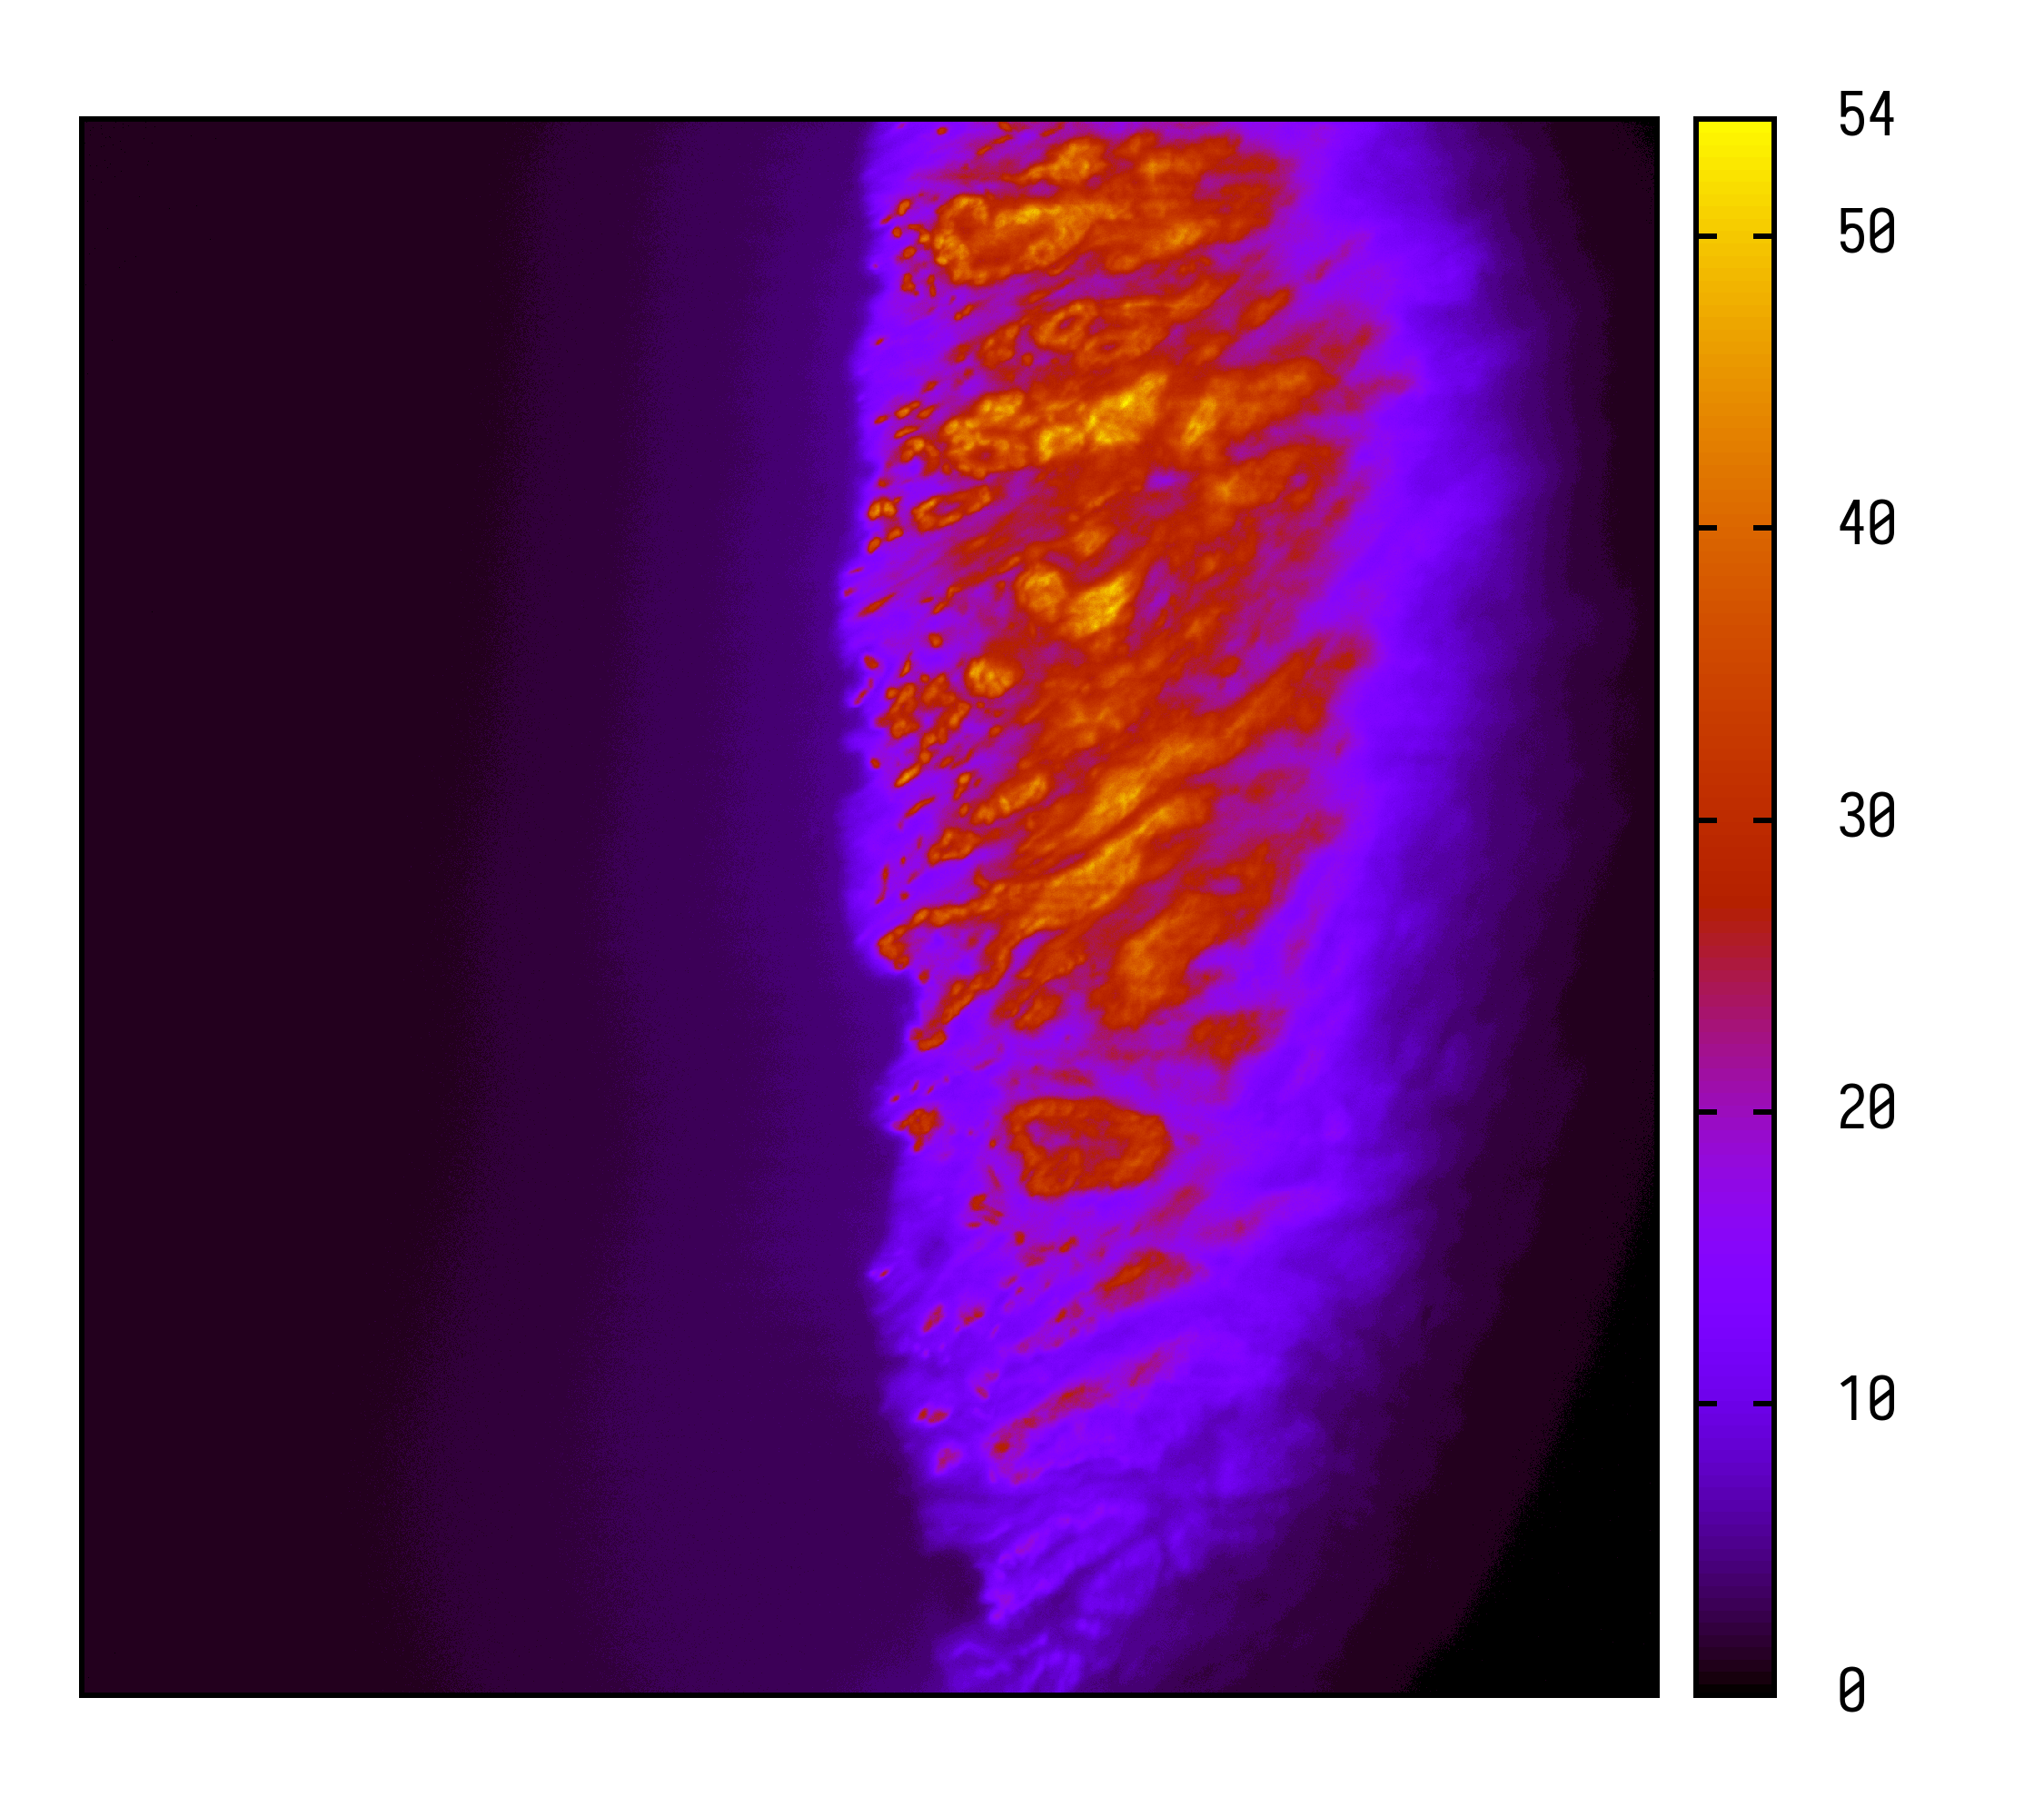
\includegraphics[width=.99\linewidth]{img/tulane_data/prostate_data_colourized.png}
                    \captionsetup{width=.8\linewidth}
                    \caption{Tissus de prostate, colorisé par \texttt{gnuplot} selon les valeurs de gris.}
                    \label{img:data:prostate_coloured}
                \end{subfigure}
            \end{tabular}
            \captionsetup{width=.8\linewidth}
            \caption{Acquisitions réalisées à l'université de Tulane, utilisées pour ce stage.}
            \label{img:data:both_prostate_samples}
        \end{figure}

        Nous pouvons voir qu'une grande partie de cette image (et plus généralement des autres images présentes dans ce jeu de données) est constituée de valeurs faibles, sur les côtés de l'échantillon. Les chercheurs à Tulane nous ont informés que lors de l'enregistrement des images, nous devions considérer les valeurs inférieures à 5 comme du bruit de fond, ne représentant pas aucune information. Ainsi, une grande partie de cette image ne contient aucune donnée significative pour notre cas d'utilisation.

        En analysant les coupes présentes dans ce jeu de données, nous pouvons voir dans la figure \ref{img:prostate:stats} que près de $70\%$ des données sont à considérer comme du bruit. La figure \ref{img:prostate:stats:repartition} représente la probabilité qu'un pixel aléatoire dans le jeu de données soit supérieur à $n$. Si l'on prend $n = 5$, nous pouvons voir que uniquement $31\%$ des données présentes représentent une information utile à la reconstruction. De plus, nous pouvons remarquer que le contraste de ces images n'est pas extrêmement élevé, ce qui pourra poser problème lorsque l'on devra faire des analyses de forme de la structure d'un échantillon.
        
        En effectuant une reconstruction partielle des images chargées en mémoire, nous pourrons donc économiser non seulement beaucoup de place mémoire, mais également raccourcir le temps nécessaire pour une reconstruction complète de l'échantillon.

        Le choix de mettre les acquisitions en format \texttt{TIFF} est judicieux, car ce format permet une grande flexibilité pour le format d'images enregistrées : il est possible d'étendre le format originel par le biais d'extensions, permettant d'enregistrer plus d'informations sous des formats quelconques, et c'est la responsabilité de l'application de lecture des images à implémenter le support de ces extensions ou non.
        
        \begin{figure}[H]
            \centering
            \begin{subfigure}{.8\linewidth}
                \centering
                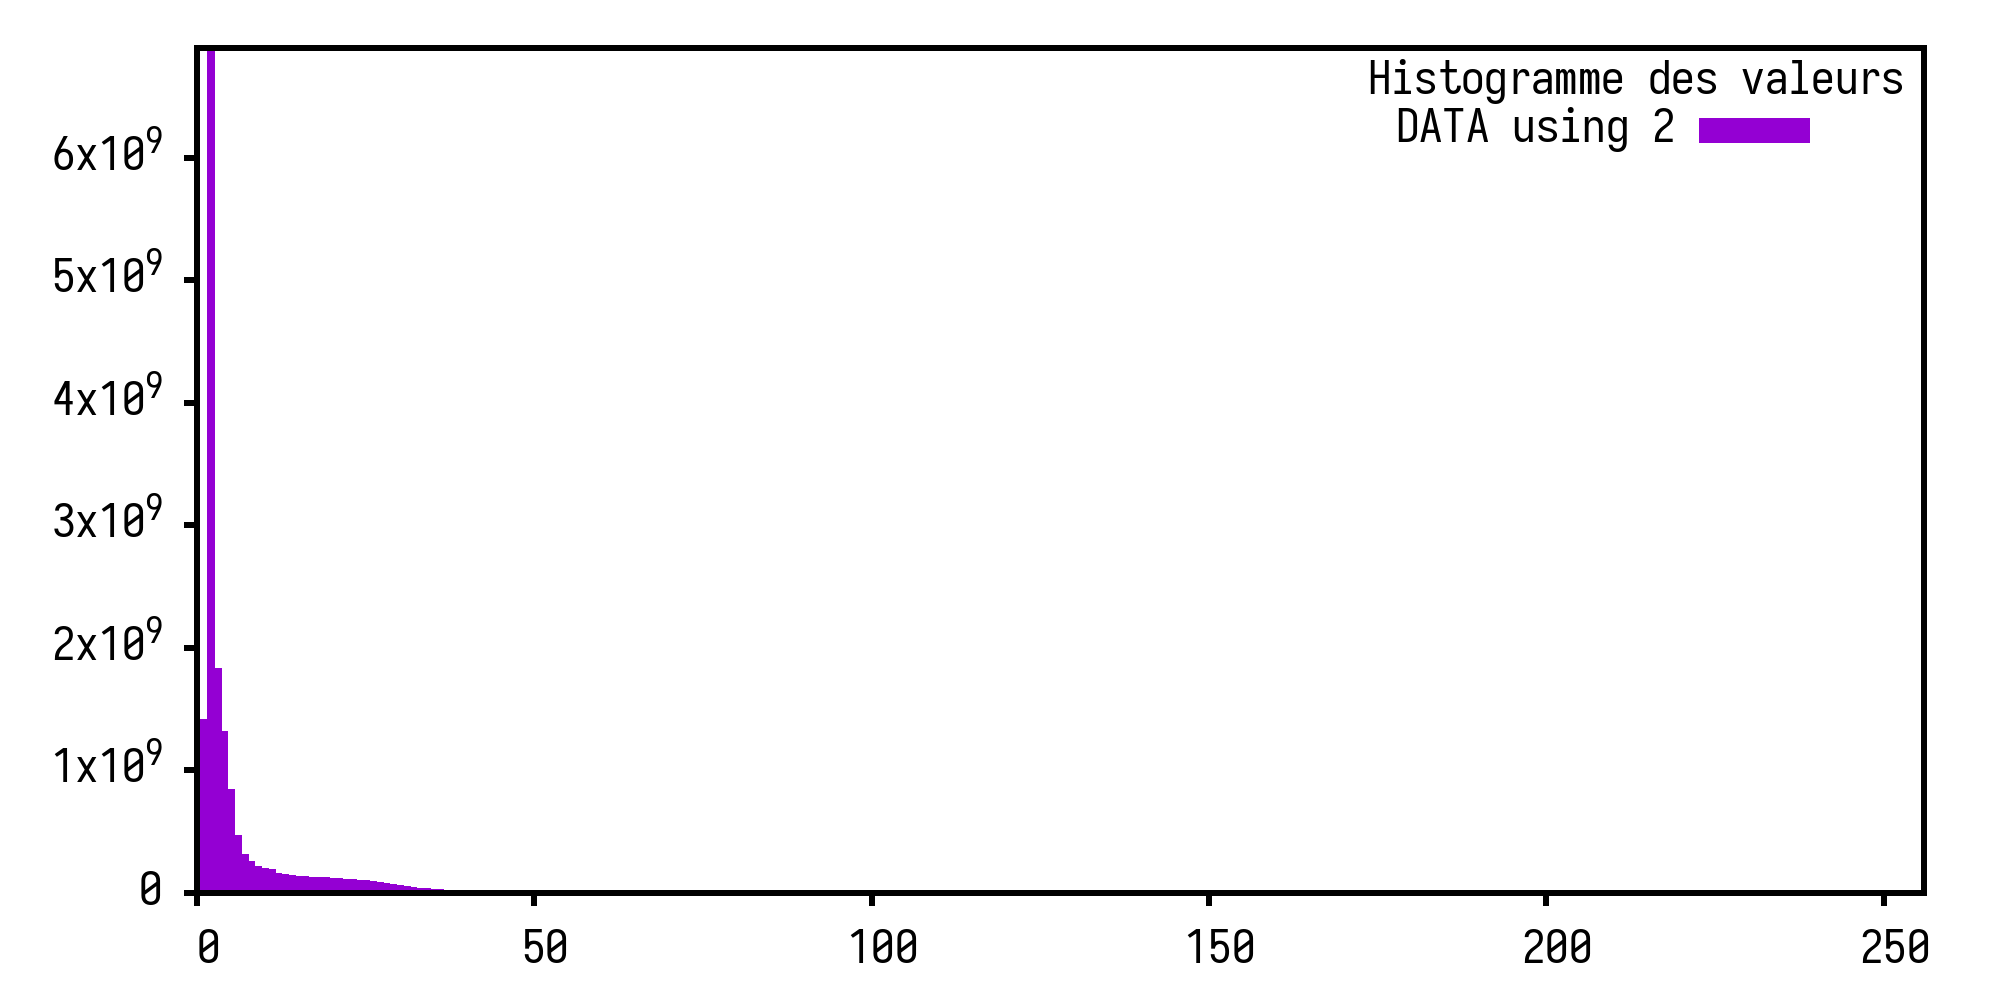
\includegraphics[width=\linewidth]{img/stats/histo.png}
                \caption{Histogramme des valeurs de niveaux de gris présentes dans le jeu de données}
                \label{img:prostate:stats:histogram}
            \end{subfigure}
            \begin{subfigure}{.8\linewidth}
                \centering
                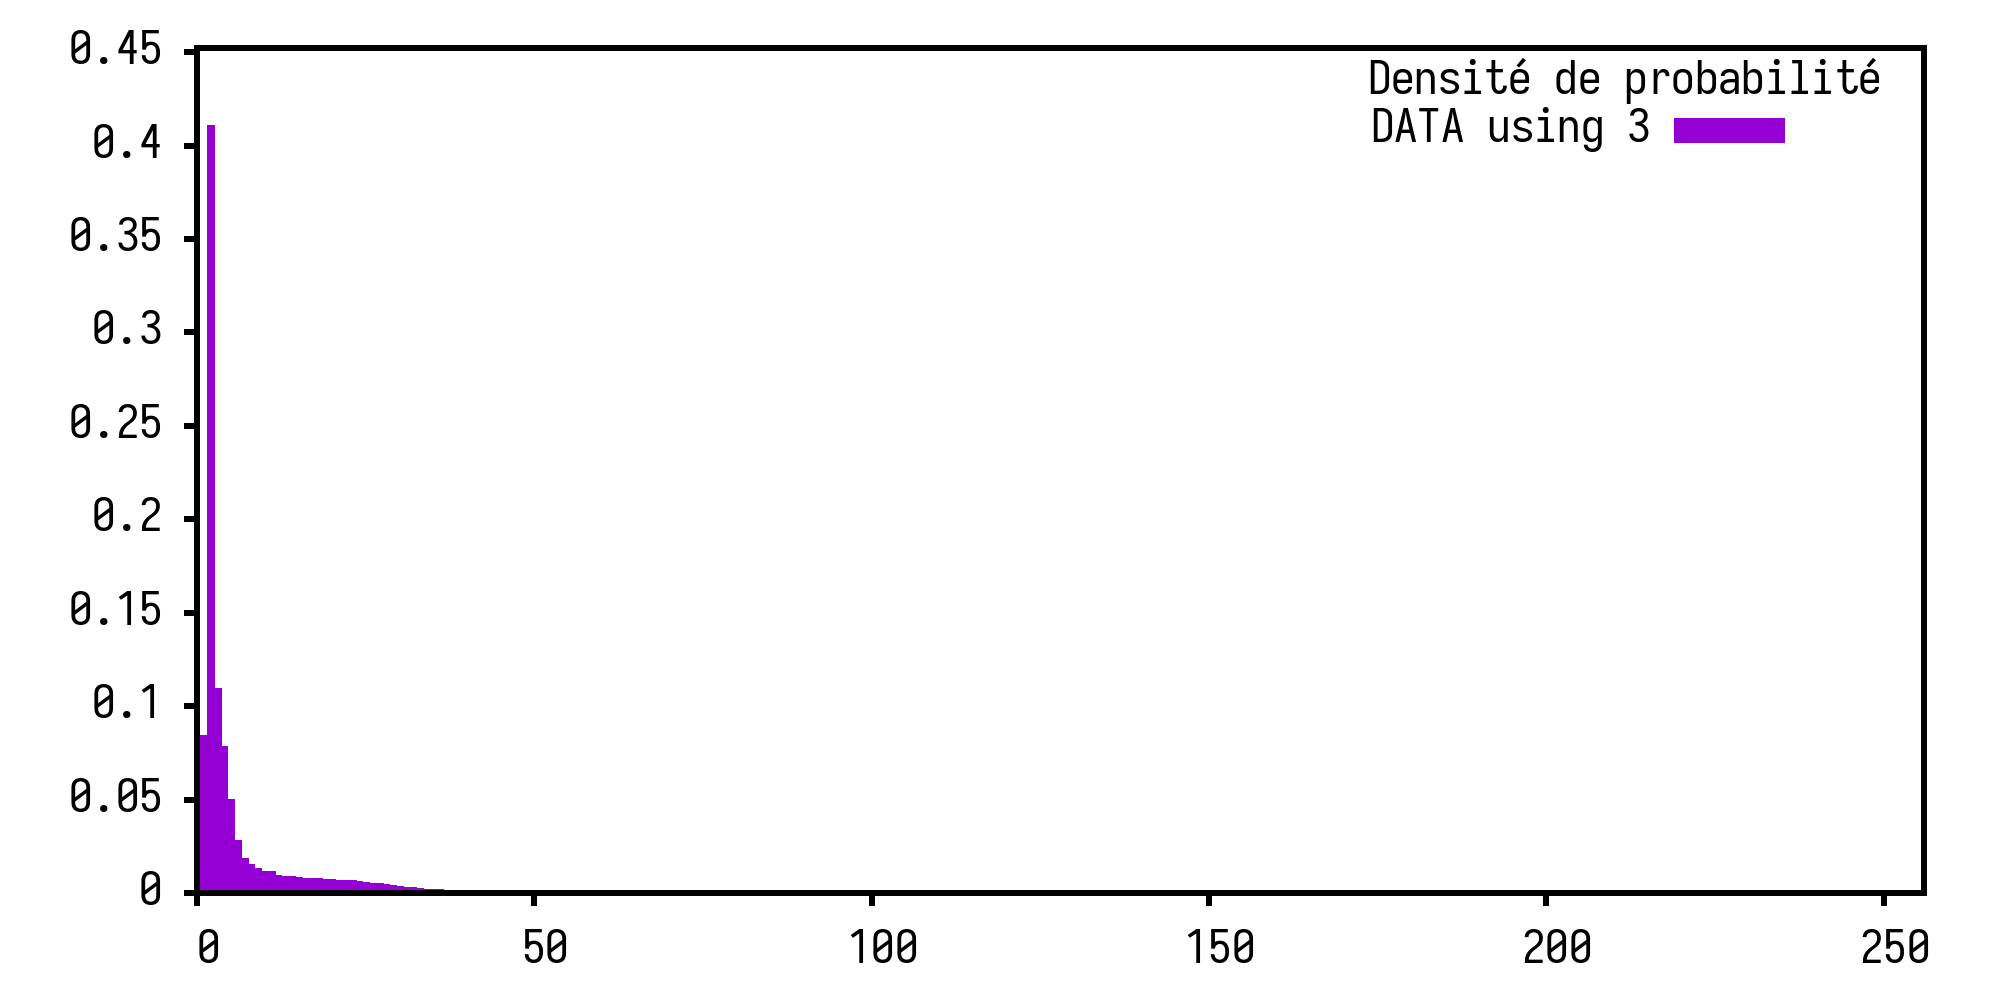
\includegraphics[width=\linewidth]{img/stats/distrib.png}
                \caption{Densité de probabilités des valeurs de niveaux de gris du jeu de données}
                \label{img:prostate:stats:ddp}
            \end{subfigure}
            \begin{subfigure}{.8\linewidth}
                \centering
                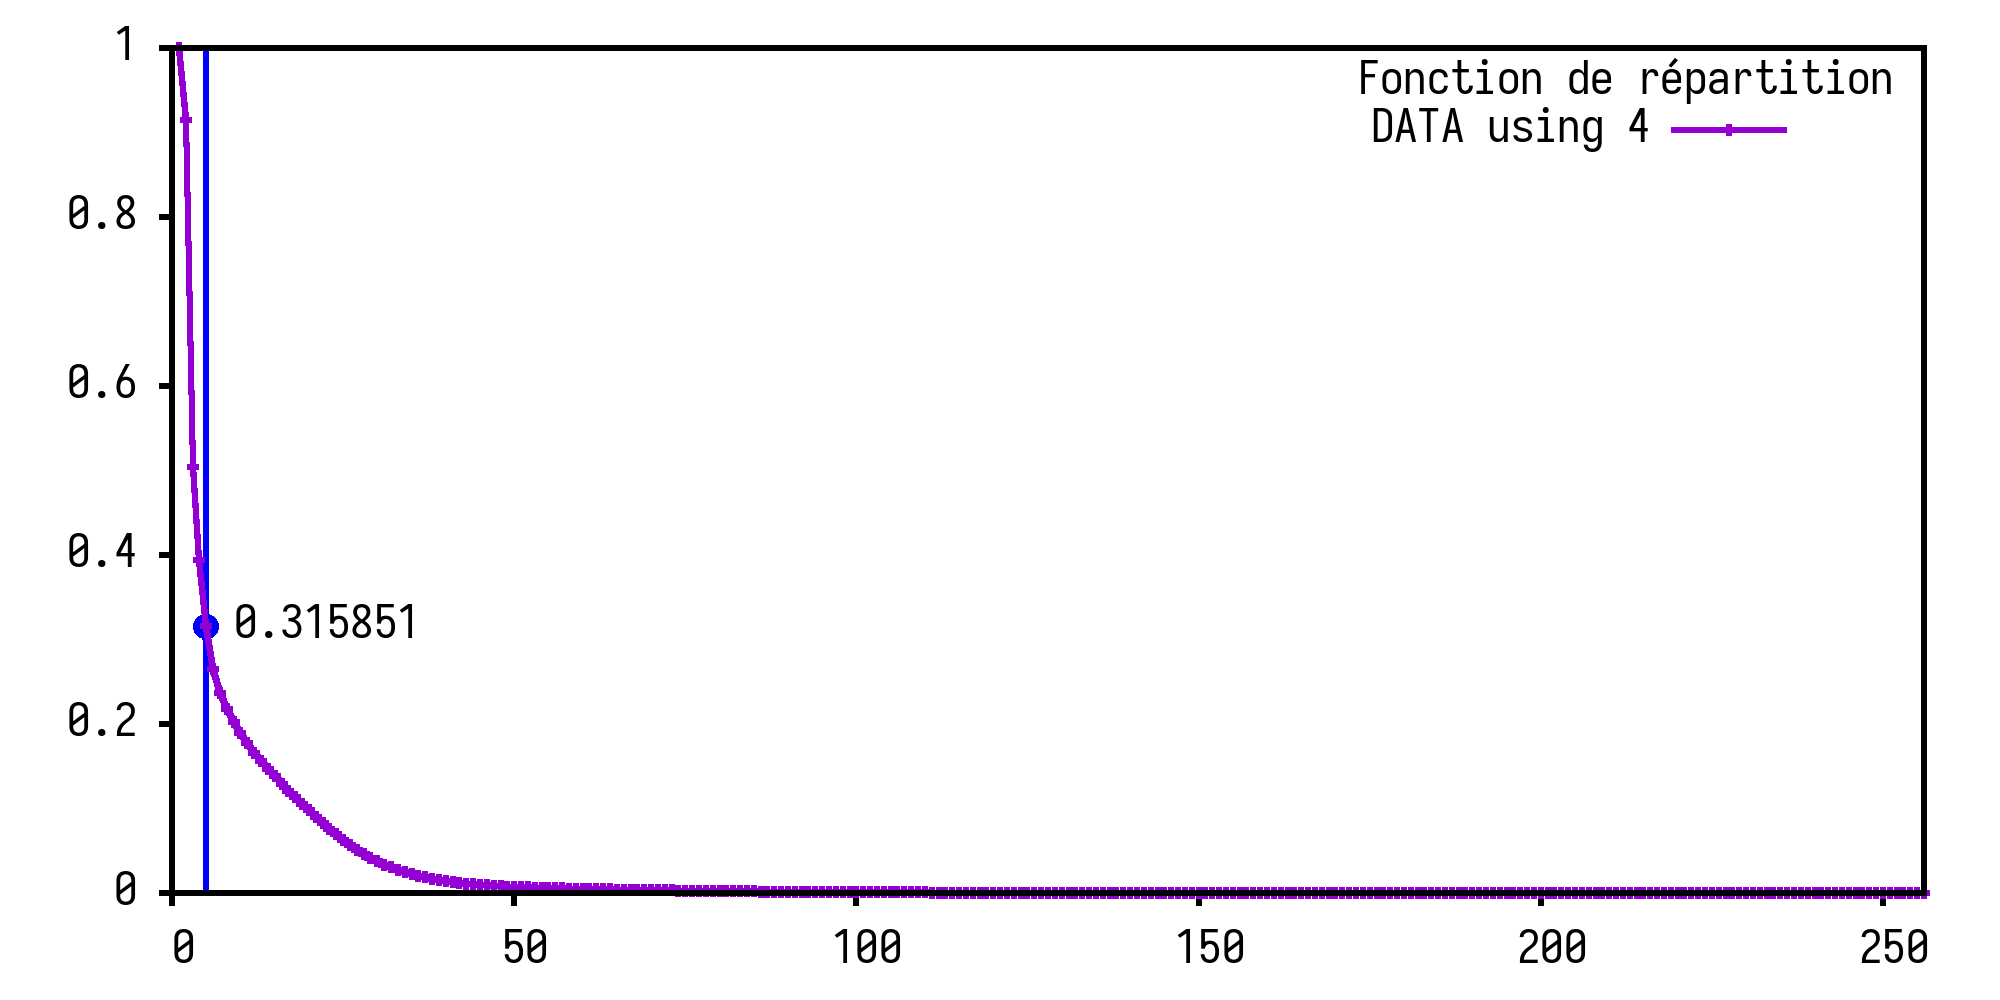
\includegraphics[width=\linewidth]{img/stats/proba.png}
                \caption{Fonction de répartition (inversée) des valeurs de niveaux de gris dans le jeux de données. La droite bleue à $x~=~5$ est permet de visualiser quelle proportion des données sont utiles dans l'acquisition de l'échantillon.}
                \label{img:prostate:stats:repartition}
            \end{subfigure}
            \captionsetup{width=.8\linewidth}
            \caption{Quelques informations sur le jeu de données fourni par Tulane}
            \label{img:prostate:stats}
        \end{figure}
        
        Une capture étant composée d'un empilement de coupes de l'échantillon de même résolution, celle-ci est donc représentée comme une image 3D, communément représentée comme une grille volumique orthonormée dont tous les éléments sont appelés \textit{voxels}, l'analogue du pixel en trois dimensions. Cette structure de données possède quelques avantages et inconvénients qui seront explorés plus en profondeur dans la section \ref{section:voxelgrid}. Cette représentation de l'acquisition de l'échantillon est une forme primaire de reconstruction 3D. Mais dans notre cas, celle-ci ne prend pas en compte les spécificités apportées par la méthode d'acquisition \textit{di-SPIM}, et ne permet pas non plus une étude de la forme des glandes dans l'échantillon car celui-ci est déformé dans son état actuel.
    }
    % }}}
    
    % Section Tulane {{{
	\section{Pré-traitement des données}\label{section:previous_tulane_work}
	{
	    %Le microscope développé par les chercheurs de l'université de Tulane permet d'effectuer une acquisition d'échantillon en utilisant la méthode \textit{di-SPIM} (détaillé en section \ref{section:microscopy}), effectuant une acquisition par coupes de l'échantillon, de manière non destructive. Chacune de ces coupes est transformée en image puis empilée avec les autres coupes de ce capteur, résultant en une image 3D. %Dans les travaux présentés ci-après dans le rapport, nous ne nous intéresserons pas au bruit présent sur le signal capturé, car la création d'un modèle de bruit ne rentre pas dans le cadre du stage.
	    
	    Dès l'arrivée des première acquisitions, les chercheurs de l'université de Tulane ont mis en place une méthode, non optimisé, de reconstruction volumique de l'échantillon. % ne prenant pas en compte les spécificités amenées par la technique de microscopie \textit{di-SPIM}. 
	    Ce processus est composé de plusieurs étapes:
	    \begin{enumerate}
	    \item "redresser" les deux piles d'images entre elles en appliquant une transformation (cisaillement, rotation, troncature) sur chacune des coupes de l'image. Comme le montre les étapes $(C)$, $(D)$ et $(E)$ de la figure \ref{img:tulane_process:reconstruction}, la décomposition de cette transformation génère une consommation mémoire importante par le stockage de résultats intermédiaires non indispensables.
	    \item re-échantillonner les deux piles d'images pour avoir une résolution uniforme. %Une copie de chaque image est faite à cette étape.
	    \item fusionner les deux piles par une opération de déconvolution à double vue~\cite{cite_deconv_richardson_lucy, cite_deconv_spim_huisken}. Cette opération permet d'améliorer la qualité et la netteté de l'image capturée, en intégrant les données des deux piles d'images. 
	    \end{enumerate}
	    	    %, indépendantes les unes des autres, est coûteux en temps de calcul et gourmand en espace disque:
	    %Ce processus est long car chacune des opérations de transformation de l'image 3D est accompagnée d'un re-échantillonnage de cette image afin de pouvoir avoir des données uniformément échantillonnées. Ces enchaînements d'interpolations suivies d'opérations complexes entraînent une explosion des quantités de données nécessaires pour stocker une acquisition complète. 
	    Chacune de ces opérations menant à une reconstruction de l'échantillon prennent plusieurs heures, et génèrent jusqu'à plusieurs téraoctets de données afin d'obtenir un résultat correct. Ces choix algorithmiques sont justifiés en grande partie par l'emploi de logiciels comme \texttt{ImageJ} ou \texttt{Amira} et de langage scriptés non optimisés tels que \texttt{Matlab} par des utilisateurs non experts. La contribution majeur de ce travail est de fournir une solution méthodologique et logicielle adaptée permettant d'effectuer ces traitements de façon économe et efficace en mémoire. De plus, notre système permet la visualisation interactive de la structure tridimensionnelle des glandes de la prostate.  % et faite à la volée, nous pouvons effectuer ces traitements plus rapidement, tout en utilisant moins de mémoire que la solution actuelle. De plus, les algorithmes étant adaptés au cas particulier de la microscopie \textit{di-SPIM}, nous pouvons conserver la morphologie complexe de l'échantillon de tissu afin de l'analyser par la suite.
	}
	    
	    \begin{figure}[h]
	        \centering
	        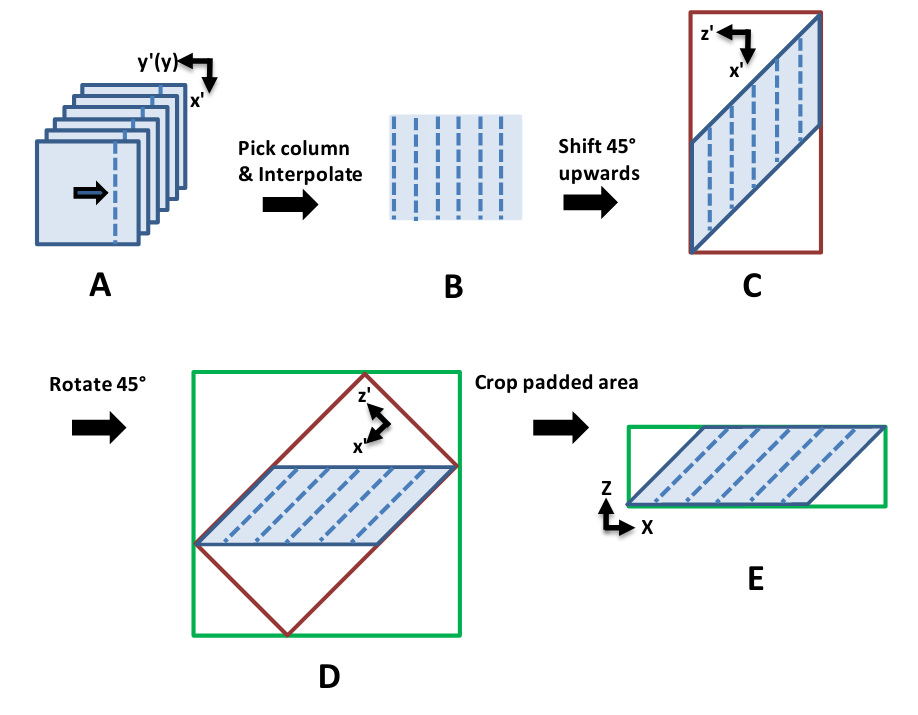
\includegraphics[width=.65\linewidth]{img/tulane_process.png}
	        \captionsetup{width=.8\linewidth}
	        \caption{Le processus actuel de reconstruction de l'université de Tulane, sans la partie de déconvolution.}
	        \label{img:tulane_process:reconstruction}
	    \end{figure}
	    
	    
    %}}}
    
}
% VIM modeline : do not touch !
% vim: set spell spelllang=fr :
